\documentclass[conference]{IEEEtran}
\usepackage{graphicx}
\usepackage{float}
\usepackage{amsmath}
%\usepackage{cite}

\begin{document}

\title{Direction of Angle Estimation}

\author{\IEEEauthorblockN{Owen Sowatzke}
\IEEEauthorblockA{\textit{Electrical Engineering Department} \\
\textit{University of Arizona}\\
Tucson, USA \\
osowatzke@arizona.edu}}
\maketitle

\begin{abstract}
	Direction of arrival (DOA) estimation plays an integral role in radar, wireless communications, sonar, radio astronomy, and navigation \cite{doa_algorithms_raghu}. Specific algorithms for DOA estimation include beamforming, MVDR, MUSIC, improved MUSIC, Root Music, and ESPRIT \cite{doa_algorithms_raghu}. Following the work of Raghu and Kamari, this paper evaulates the performance of each of these direction of arrival algorithms operating on data from a uniform linear array. 
\end{abstract}

	\section{Background}
	
	Each of the direction of angle algorithms compared in this report operate on data collected with an antenna array. This report specifically examines data collected with a uniform linear array (ULA). A block diagram of a uniform linear array with $M$ antenna elements, receiving signals from $D$ sources is given by Raghu and Kamari in \cite{doa_algorithms_raghu}.
	
	\begin{figure}[H]
		\centerline{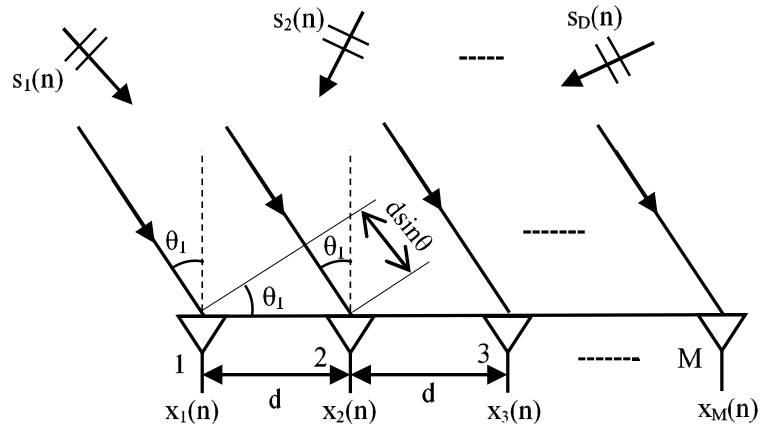
\includegraphics[width=0.5\textwidth]{uniform_linear_array.png}}
		\caption{Uniform Linear Array \cite{doa_algorithms_raghu}}
		\label{Monte Carlo Estimate}
	\end{figure}
	
	As shown in the figure above, let $d$ be the distance between successive array elements, and $\beta$ be defined as $2\pi/\lambda$. Then if each of the source signals is given as $s_1(n),...,s_D(n)$, the signal received by m-th array element can be written as:
	%
	\begin{equation}
		\label{received_signal}
		\begin{split}
			x_m(n) &= s_1(n)e^{-j{\beta}d(m-1)\sin{\theta_1}} + \cdots\\
			&+ s_D(n)e^{-j{\beta}d(m-1)\sin{\theta_D}} + w_m(n)
		\end{split}
	\end{equation}
	%
	where $w_m(n)$ denotes the noise on the m-th element \cite{doa_algorithms_raghu}.
	
	Equation (\ref{received_signal} can be rewritten in matrix form as follows:
	%
	\begin{equation}
		X = AS + W
	\end{equation}
	%
	where $X = \begin{bmatrix} x_1(n) & \cdots & x_n(n)\end{bmatrix}^T$ is the Mx1 received signal vector, $A$ is the MxD array steering matrix, $S = \begin{bmatrix} s_1(n) & \cdots & s_D(n)\end{bmatrix}^T$ is the Dx1 source signal vector, and $W = \begin{bmatrix} w_1(n) & \cdots & w_n(n)\end{bmatrix}^T$ is the Mx1 noise signal vector \cite{doa_algorithms_raghu}. The array steering matrix $A$ can be written as:
	%
	\begin{equation}
		A = \begin{bmatrix} a(\theta_1) & \cdots & a(\theta_D) \end{bmatrix}
	\end{equation}
	%
	where $a(\theta_i)$ represents the Mx1 array response for the source signal incident at angle $\theta_i$ and is defined in \cite{doa_algorithms_raghu} as:
	%	
	\begin{equation}
		\label{array_response_vector}
	 	a(\theta_i) = \begin{bmatrix} 1 & e^{j{\beta}d\sin(\theta_i)} & \cdots & e^{j{\beta}d(M-1)\sin(\theta_i)}\end{bmatrix}^T
	\end{equation}
	
		Each direction of arrival algorithm leverages spatial auto-correlation matrices $R_{xx}$ defined in \cite{doa_algorithms_raghu}  using the received signal vector $X$ as:
	%
	\begin{equation}
		R_{xx} = E[XX^H]
	\end{equation}
	%
	The expected value in the above equation is estimated using $K$ (a finite number) samples of the received signal vector $X$. The resulting spatial auto-correlation estimate ${R}_{xx}$ is given in \cite{doa_algorithms_raghu} as follows: 
	%
	\begin{equation}
		\label{spatial_matrix_estimate}
		\hat{R}_{xx} = \sum_{n=1}^{K}{X(n)X^H(n)}
	\end{equation}
	
	\section{Direction of Arrival Algorithms}
	
	\subsection{Beamforming}
	
		Beamforming uses the estimate of the spatial auto-correlation matrix $\hat{R}_{xx}$ defined in Equation (\ref{spatial_matrix_estimate}) to estimate the spatial spectrum $\hat{P}_{bf}(\theta)$ \cite{doa_algorithms_raghu}. The spatial spectrum estimate $\hat{P}_{bf}(\theta)$ is defined by
		%
		\begin{equation}
			\hat{P}_{bf}(\theta) = a^H(\theta)\hat{R}_{xx}a(\theta)
		\end{equation}
		%
		where $a(\theta)$ is the array response given in Equation (\ref{array_response_vector}).
		
		To estimate the direction of arrival, compute the spatial spectrum in discrete steps over a region of interest. Then, find the peaks of the spatial spectrum. The angles corresponding to the peaks are the directions of arrival for each source.
		
	\subsection{Capon/MVDR}
	
		The Capon algorithm seeks to minimize the power of received signals in all direction except for the look angle \cite{doa_algorithms_raghu}. The Capon spatial spectrum $\hat{P}_{capon}(\theta)$ is generated using  the spatial auto-correlation matrix estimated by Equation (\ref{spatial_matrix_estimate}). For each look angle $\theta$, the spatial spectrum is given by:
	%
	\begin{equation}
		\hat{P}_{capon}(\theta) = \frac{1}{a^H(\theta){\hat{R}_{xx}}^{-1}a(\theta)}
	\end{equation}
	%
	
		Similar to beamforming direction of arrival estimation, Capon direction of angle estimation requires generating the spatial spectrum in discrete steps over a region of interest. Then, this spectrum can be searched for peaks. The angle corresponding to the peaks are the directions of arrival for each source.
	
	\subsection{MUSIC}
	
		The Multiple Signal Classification (MUSIC) algorithm takes an eigen-decomposition of the spatial auto-correlation matrix to produce orthogonal signal and noise subspaces. The eigenvectors of the resulting noise subspace are used to generate a spatial spectrum which can be used to estimate the directions of arrival \cite{doa_algorithms_raghu}.
	
		To find the signal and noise subspaces, the spatial auto-correlation matrix must decomposed into its eigenvalues and eigenvectors:
	%
	\begin{equation}
		\hat{R}_{xx} = E{\Lambda}E^H
	\end{equation}
	%
	In the above equation, $\Lambda = \text{diag}\{\lambda_0,...,\lambda_{M-1}\}$ is the MxM diagonal eigenvalue matrix and $E=\{e_0,...,e_{M-1}\}$ is the MxM eigenvector matrix. If the eigenvalues are sorted in ascending order (i.e. $\lambda_0 < ... < \lambda_{M-1}$), then the $D$ smallest eigenvalues $\{\lambda_0,...,\lambda_{D-1}\}$ and their corresponding eigenvectors $\{e_0,...,e_{D-1}\}$ correspond to the noise subspace.
	
	The number of source signals $D$ is typically not known, but can be estimated using a variety of methods, which include AIC and MDL \cite{num_sources_est_salman}. Both of these algorithms require a flipped copy of the eigenvalues such that $\lambda_0 > ... > \lambda_{M-1}$. Using the flipped eigenvalues, the number of sources estimated with AIC is given in \cite{num_sources_est_salman} as
	%
	\begin{equation}
		\begin{split}
		N_{AIC} &= argmin_n\left(-2\log\left(\frac{\prod_{i=n}^{M-1}{{\lambda_i}^{\frac{1}{M-k}}}}{\frac{1}{M - n}\sum_{i=n}^{M-1}{\lambda_i}}\right)^{(M-n)K}\right. \\
		& \left. + 2n(2M - n) \vphantom{-2\log\left(\frac{\prod_{i=n}^{M-1}{{\lambda_i}^{\frac{1}{M-k}}}}{\frac{1}{M - n}\sum_{i=n}^{M-1}{\lambda_i}}\right)^{(M-n)K}} \right)
		\end{split}
	\end{equation}
	where $n$ is the index of each eigenvalue.
	%\begin{equation}
	%	A = \begin{bmatrix}
	%		1 & 1 & \cdots & 1\\
	%		e^{j{\beta}d\sin{\theta_1}} & e^{j{\beta}d\sin{\theta_2}} & \cdots & e^{j{\beta}d\sin{\theta_D}} \\
	%		\vdots & \vdots & \ddots & \vdots\\
	%		e^{j{\beta}d(M-1)\sin{\theta_1}} & e^{j{\beta}d(M-1)\sin{\theta_2}} & \cdots & e^{j{\beta}d(M-1)\sin{\theta_D}}
	%	\end{bmatrix}
	%\end{equation}
	\bibliographystyle{IEEEtran}
	\bibliography{IEEEabrv,sources}
\end{document}